\documentclass{article}

\usepackage[dvipsnames]{xcolor}%barevne rozliseni kodu
\usepackage{mathptmx}
%packages for language
\usepackage[czech]{babel}
\usepackage[utf8]{inputenc}
%packages for graphic
\usepackage{graphicx}
\usepackage{pgfplots}
\usepackage{pgfplotstable}
\usepackage{multirow}
\usepackage{tikz}
\usepackage{import}
\usepackage[a4paper, total={17cm,25.7cm}, top=2cm, left=2cm, includefoot]{geometry}
\usepackage{todonotes}
\usepackage{standalone}
\usepackage{colortbl}%pro barevne zmeny v tabulce
\usepackage{float}
\usepackage{csvsimple} %pro import a práci s csv soubory
\usepackage{indentfirst}  % odsazení prvního řádku v odstavci
\usepackage{hyperref} %dela odkazy na mista v dokumentu atd
\usepackage{amsmath}%psani matic
\usepackage{mathrsfs}%psani kroucenym matematickym pismem
\usepackage{pdfpages}%vkladani celych pdf dokumentu
%cesta k obrazkum: ./Graphics/....
%\usepackage[utf8]{inputenc}
\usepackage{listings,lstautogobble}
\usepackage{mathtools}
\usepackage{svg}
\usepackage{float}
\usepackage{amssymb}
\usepackage{scalerel}
%\usepackage{romannum}

%nastaveni parametru pro jazyk Matlab a jeho font a syntaxi v listing
\lstset{language=Matlab,%
	%basicstyle=\color{red},
	breaklines=true,%
	morekeywords={matlab2tikz},
	keywordstyle=\color{blue},%
	morekeywords=[2]{1}, keywordstyle=[2]{\color{black}},
	identifierstyle=\color{black},%
	stringstyle=\color{Purple},
	commentstyle=\color{ForestGreen},%
	showstringspaces=false,%without this there will be a symbol in the places where there is a space
	numbers=left,%
	numberstyle={\tiny \color{black}},% size of the numbers
	numbersep=9pt, % this defines how far the numbers are from the text
	emph=[1]{for,end,break},emphstyle=[1]\color{red}, %some words to emphasise
	%emph=[2]{word1,word2}, emphstyle=[2]{style},
	autogobble = true%zarovnani doleva
}


\begin{document}
	\begin{titlepage}
    \begin{center}
        \LARGE
        Západočeská Univerzita v Plzni\\
        Fakulta Aplikovaných Věd\\
        
        \vspace{1cm}
        
        \includegraphics[width=0.5\textwidth]{./Graphics/FAV_logo.pdf}
        
        \vspace{4cm}
        
        \textbf{Semestrální práce z předmětu URM}
        
        \vspace{0.5cm}
        Filip Jašek, David Žahour
        
    \end{center} 
    \vfill
        \noindent
        \large
        Předmět: KKY/URM (Úvod do Robotiky a Mechatroniky)\\
        Přednášející: Ing. Martin Švejda, Ph.D.\\
        Cvičící: Ing. Arnold Jáger \hfill Datum: \today
\end{titlepage}
	\tableofcontents
	\newpage
	\section{Glóbus}
		\subsection{Zadání}
			Na glóbusu vykreslete cestu ze Singapuru do New Yorku. Do obou měst zapíchněte špendlík který bude vycházet ze středu zeměkoule. Souřadnice destinací jsou následující. 
			\begin{table}[H]
				\begin{tabular}{|c|c|c|}
					\hline
					Město (letiště) & Délka & Šířka \\
					\hline
					\textbf{Singapur (SIN)} &  \(103.986306^{\circ}\) & \(1.351652^{\circ}\) \\
					\hline
					\textbf{New York (EWR)} & \(-74.168944^{\circ}\) & \(40.690093^{\circ}\) \\
					\hline
				\end{tabular}
				\label{tab:1:souradnice}
				\centering
			\end{table}
		\subsection{Postup řešení}
			Využijeme toho že zeměpisnou délku a šířku lze považovat za výchylku vůči 0 poledníku a rovníku. K samotnému výpočtu využijeme skládání homogenních transformačních matic. Pro usnadnění výpočtů budeme brát poloměr zeměkoule roven 1.  
				\begin{lstlisting}[caption={Použité funkce v MATLABu},label={lst:sql}]
					%rotace kolem osy Z
					function Rz = rotZ(x)
					Rz = [cos(x),-sin(x),0;
					sin(x),cos(x) ,0;
					0     ,0      ,1];
					end
					
					%rotace kolem osy Y
					function Ry = rotY(x)
					Ry = [cos(x) ,0,sin(x);
					0       ,1,0      ;
					-sin(x),0,cos(x)];
					end
					
					%translace v ose X
					function Tx = translX(x)
					Tx = [1,0,0,x;
					0,1,0,0;
					0,0,1,0;
					0,0,0,1];
					end
				\end{lstlisting}
			Po zavolání těchto funkcí dostaneme k dispozici jednotlivé rotační matice které následně přenásobíme a vznikne nám následující homogenní transformační matice. 
				\begin{equation*}
					T_v^0 = rotZ(\alpha) * rotY(-\beta) *translX(r)
				\end{equation*}
			Po dosazení a vypočtení dostaneme následující matici, ze které vyčteme až poslední sloupec který nám udává kartézské souřadnice měst.
				\begin{align}
					T^0_v &= \begin{bmatrix}
						\multicolumn{3}{c}{} & \color{red} t_x \\
						\multicolumn{3}{c}{\scaleobj{2}{R}} & \color{red} t_y \\ 
						\multicolumn{3}{c}{} & \color{red} t_z \\
						0 & 0 & 0 & 1 \\
					\end{bmatrix} \label{eq:trans_mat_final} \\   
				\end{align}
			\newpage
			\subsubsection{Zobrazení špendlíku}
				K vykreslení špendlíku použijeme následující kód. 
					\begin{lstlisting}[caption={Výpočet a vykreslení špendlíků.},label={lst:sql}]
						%% vykresleni [Singapuru,NewYorku]
						delka = [103.986306,-74.168944];
						sirka = [1.351652,40.690093];
						polomer = 1;
						%vytvoreni prazdne transformacni matice bez deformaci a zmeny velikosti
						transfMAT = zeros(4);
						transfMAT(end,end) = 1;
						for i=1:2
						%vypocet matice rotace
						R2 = rotZ(delka(i))*rotY(-sirka(i));%*transY(polomer)
						%vypocet translacni matice
						translMAT = translX(polomer);
						% doplneni do vysledne transformacni matice
						Tv = transfMAT;
						Tv(1:3,1:3) = R2;
						Tvsave = Tv;
						Tv = Tv*translMAT;
						
						%docasne ulozeni pocatecnich souradnic spendliku
						vectX=[Tv(1,4),0];
						vectY=[Tv(2,4),0];
						vectZ=[Tv(3,4),0];
						
						% posunuti kvuli vektoru spendliku
						% vektor spendliku je dlouhy 1/4 polomeru spendliku
						translMAT = translX(polomer/4);
						Tv = Tv*translMAT;
						
						% docasne ulozeni konncovych souradnic spendliku, kde se zaroven
						% nachazi hlavicka spendliku
						vectX(2) = Tv(1,4);
						vectY(2) = Tv(2,4);
						vectZ(2) = Tv(3,4);
						
						% vykresleni spendliku
						plot3([vectX(1) vectX(2)], [vectY(1) vectY(2)], [vectZ(1) vectZ(2)],'Color','k','LineWidth',2.5)
						plot3(Tv(1,4),Tv(2,4),Tv(3,4),'ro','MarkerFaceColor','r','MarkerSize',9)
						end
					\end{lstlisting}
			\newpage
			\subsubsection{Výpočet cesty}
				K výpočtu rozdělíme cestu z počáteční nulové polohy do výsledné pozice dané zeměpisnými souřadnicemi na 100 kroků a pro každý krok vypočteme výsledek následujícího kódu pro zadanou polohu. Získáme tak 100 bodů ve 3D prostoru jejímž spojením dosáhneme výsledné cesty.
					\begin{lstlisting}[caption={Výpočet polohy na globu v souřadnicích \(x\ ,y\ ,z\)},label={lst:bod_na_globu}]
						function [Gx,Gy,Gz] = pointOnGlobe(d,s,r)
						% d-zemepisna delka
						% s-zemepisna sirka
						% r-polommer modelu zemekoule
						% vytvoreni prazdne  transformacni matice, ktera nedeformuje perspektivu a
						% zachovava velikost
						transfMAT = zeros(4);
						transfMAT(end,end) = 1;
						% vytvoreni matice rotace postupnou rotaci kolem osy Z a potom kolem osy Y
						% tzn: nejdrive nastaveni zemepisne sirky a pote delky
						R2 = rotZ(d)*rotY(-s);
						%vypocet translacni matice pro pozdejsi nasobeni a ziskani souradnic na
						%povrchu Zemekoule
						translMAT = translX(r);
						% doplneni do vysledne transformacni matice
						Tv = transfMAT;
						Tv(1:3,1:3) = R2;
						Tv = Tv*translMAT;
						Gx = Tv(1,4);
						Gy = Tv(2,4);
						Gz = Tv(3,4);
						end
					\end{lstlisting}
			\subsubsection{Výpočet nejkratší cesty}
				K výpočtu nejkratší cesty využijeme příkaz \verb|gcwaypts| které nám opět vrátí diskretizované body cesty v zeměpisných souřadnicích, které funkcí \ref{lst:bod_na_globu} transformujeme na souřadnice ve 3D prostoru.\\
				
				Příkaz \verb|gcwaypts| hledá nejkratší cestu na kulovém povrchu nalezením kružnice se středem totožným se středem koule s oběma body náležící této kružnici. Menší část obvodu kružnice mezi dvěma zadanými body je hledanou nejkratší cestou.
		\subsection{Výsledky}
			\begin{figure}[H]
				\centering
				\includegraphics[width=\textwidth]{./Graphics/1_Graphics/globus.eps}
				\caption{Aproximovaný model Zeměkoule s vykreslenými špendlíky v místech zadaných měst spolu s cestami pomocí skládání homogenních transformačních matic (červeně) a nejkratší cestou (žlutě).}
				\label{pic:1_globus}
			\end{figure}
		\subsection{Závěr}
			Byli jsme schopní využít transformačních matic k převodu zeměpisných souřadnic do kartézských souřadnic a zároveň vypočítat cestu mezi dvěma body na zeměkouli zadanými zeměpisnými souřadnicemi. 
	\newpage
	\section{Přímý a inverzní geometrický model}
		\label{section:2}
		\subsection{Zadání}
			Máme za úkol pomocí Denavit Hartenbergovy úmluvy vytvořit geometrický model manipulátoru. Dále pomocí geometrického modelu vyřešit přímou geometrickou úlohu \textbf{DGM} (z natočení kloubů manipulátoru získat polohu koncového efektoru). Dále vyřešit inverzní geometrickou úlohu \textbf{IGM}, kdy z polohy konc. ef. zjistíme nastavení kloubů ramen. Toto vše vytvořit jako model v prostředí simulink. S možností ověření jak DGM tak IGM.  
				\begin{figure}[H]
					\centering
					\includegraphics[width=\textwidth]{./Graphics/2_Graphics/manipulator_kresba.pdf}
					\caption{Model manipulátoru}
					\label{pic:2_manipulator_kresba}
				\end{figure}
		\subsection{Postup řešení}
			\subsubsection{Geometrický popis}
				Pro popsání manipulátoru se využije D-H úmluva která má pouze 4 parametry pro přechody mezi souřadnicovými soustavami manipulátoru. D-H úmluva má výhodu v tom, že jí lze algoritmizovat. 
					\begin{table}[H]
						\begin{tabular}{|c|c|c|c|c|}
							\hline
							Kloub & \(d_i\) & \(\theta_i\) & \(a_i\) & \(\alpha_i\) \\
							\hline
							1 & \(0\) & \(\theta_1\) & \(a_1\) & \(0\) \\
							\hline
							2 & \(0\) & \(\theta_2\) & \(a_2\) & \(0\) \\
							\hline
							3 & \(0\) & \(\theta_3\) & \(a_3\) & \(0\) \\
							\hline
						\end{tabular}
						\centering
						\caption{D-H pro zadaný manipulátor.}
						\label{tab:dh_params}
					\end{table}
				\newpage
				Záznamy jednotlivých parametrů:
				
					\begin{enumerate}
						\item \(a_i\) - Kolmá vzdálenost os \(z_i\) a \(z_{i-1}\).
						\item \(d_i\) - Kolmá vzdálenost os \(x_{i}\) a \(x_{i-1}\). 
						\item \(\alpha_i\) - Úhel natočení mezi osy \(z_i\) a \(z_{i-1}\).
						\item \(\theta_i\) - Úhel natočení mezi osy \(x_i\) a \(x_{i-1}\).
					\end{enumerate}
			\subsubsection{DGM}
	
				D-H parametry nám dávají možnost vytvoření transformačních matic kdy transformační matice z kloubu \(i-1\) do \(i\) bude mít tuto podobu.
					\begin{align}
						T^{i-1}_i &= T_{rot\_z} \cdot T_{trans\_x} \\
						T^{i-1}_i &= \begin{bmatrix}
							cos\theta_i & -sin\theta_i & 0 & a_i \cdot cos\theta_i \\
							sin\theta_i & cos\theta_i & 0 & a_i \cdot sin\theta_i \\
							0 & 0 & 1 & 0 \\
							0 & 0 & 0 & 1 \\
						\end{bmatrix} \\
						\intertext{Po dosazení našich parametrů dostaneme:}
						T^0_1 &= \begin{bmatrix}
							c_1 & -s_1 & 0 & a_1c_1 \\
							s_1 & c_1 & 0 & a_1s_1 \\
							0 & 0 & 1 & 0 \\
							0 & 0 & 0 & 1 \\
						\end{bmatrix} \label{eq:dgm:t_individual} \\
						T^1_2 &= \begin{bmatrix}
							c_2 & -s_2 & 0 & a_2c_2 \\
							s_2 & c_2 & 0 & a_2s_2 \\
							0 & 0 & 1 & 0 \\
							0 & 0 & 0 & 1 \\
						\end{bmatrix} \nonumber \\
						T^2_3 &= \begin{bmatrix}
							c_3 & -s_3 & 0 & a_3c_3 \\
							s_3 & c_3 & 0 & a_3s_3 \\
							0 & 0 & 1 & 0 \\
							0 & 0 & 0 & 1 \\
						\end{bmatrix} \nonumber \\
						\intertext{Pro zjednodušení zápisu využíváme:}
						s_i &= sin(\theta_i) \\
						c_i &= cos(\theta_i) \nonumber
					\end{align} 
				Chceme-li získat pozici koncového efektoru, tak je potřeba transformační matice vynásobit. 
			
					\begin{align}
						T^0_3 &= T^0_1 \cdot T^1_2 \cdot T^2_3 \\
						\intertext{Po vynásobení a zjednodušení matice dostáváme tuto podobu:}
						T^0_3 &= \begin{bmatrix}
							c_{123} & -s_{123} & 0 & a_1c_1 + a_2c_{12} + a_3c_{123} \\
							s_{123} & c_{123} & 0 & a_1s_1 + a_2s_{12} + a_3s_{123} \\
							0 & 0 & 1 & 0 \\
							0 & 0 & 0 & 1 \\
						\end{bmatrix} \label{eq:dgb_trans_mat_final} \\
					\end{align}
				\textbf{DGM} lze chápat jako funkci kloubových souřadnic \(\mathbb{Q}\) a vektor délek ramen \(\xi\)
					\begin{align}
						\mathbb{X} &= \mathbb{F}(\mathbb{Q}), \label{eq:dgm_eq_gen} \\
						\textnormal{resp.  } \mathbb{X} &= \mathbb{F}(\mathbb{Q}, \xi) \nonumber\\
					\end{align}
				Cílem DGM je z pozice natočení jednotlivých kloubů získat finální pozici a natočení koncového efektoru ten získáme z posledního sloupce matice $T^0_3$. Úhel natočení je roven součtu všech kloubových souřadnic z transformační matice ho získáme pomocí funkce \(arctan2\).
					\begin{align}
					\mathbb{F} &= \begin{bmatrix}
					  	 a_1c_1 + a_2c_{12} + a_3c_{123} \\
					     a_1s_1 + a_2s_{12} + a_3s_{123} \\
					  	\arctan2({s_{123}}, {c_{123}}) \\
					\end{bmatrix} \label{eq:dgm:f}
					\end{align}
				Toto nám představuje řešení DGM 
			\subsubsection{IGM}
				Inverzní geometrická úloha, jak říká název, představuje snahu ze zadané pozice koncového efektoru získat úhly pro jednotlivá ramena manipulátoru. 
					\begin{align}
						\textnormal{resp.}\quad \mathbb{Q} &= \mathbb{F}^{-1}(\mathbb{X}, \xi) \nonumber \\
						\intertext{z předchozí části víme} 
						\begin{bmatrix}
							x \\
							y \\
							\varphi \\
						\end{bmatrix} &= \begin{bmatrix}
							a_1c_1 + a_2c_{12} + a_3c_{123} \\
							a_1s_1 + a_2s_{12} + a_3s_{123} \\
							\theta_1 + \theta_2 + \theta_3 \\
						\end{bmatrix} 
						\intertext{Po úpravách dostaneme }
						(x-a_3c_{123})^2 + (y-a_3s_{123})^2 &= a_2^2 + 2a_1a_2c_2+a_1^2 	\label{eq:igm:soust_upr}\\
						\intertext{,stále platí}
						c_{123} = c_\varphi &= \cos(\theta_1 + \theta_2 + \theta_3) \nonumber \\
						s_{123} = s_\varphi &= \sin(\theta_1 + \theta_2 + \theta_3) 
					\end{align}
				Následně ze vztahů vyjádříme jednu ze složek vektoru $ \mathbb{Q} $  konkrétně $\theta_2$. Nejdříve získáme výraz cos($\theta_2$) a pro tu následně dokážeme získat i hodnotu sin($\theta_2$). Pomocí těchto 2 složek následně získáme hodnotu $\theta_2$ kde k tomu využiji funkce \(arctan2\). 
				
					\begin{align}
						\cos(\theta_2) &= \frac{(x-a_3c_{123})^2+(y-a_3s_{123})^2-a_1^2-a_2^2)}{2a_1a_2} \label{eq:igm:c2} \\
						\sin(\theta_2) &= \pm \sqrt{1-\cos^2(\theta_2)} \label{eq:igm:s2} \\
						\theta_{21} &= \arctan2(+\sin(\theta_2), \cos(\theta_2)) \label{eq:igm:theta_2_final}\\
						\theta_{22} &= \arctan2(-\sin(\theta_2), \cos(\theta_2))
					\end{align}
				
				\noindent Jak můžeme vidět dostáváme dvě řešení rovnice. dále potřebujeme získat zbývající 2 složky vektoru \(\mathbb{Q}\). 
				Pro jejich získání upravíme původní soustavu rovnic.
				
					\begin{align}
						x-a_3c_{123} &= a_2(c_1c_2-s_1s_2)+a_1c_1 \nonumber \\
						x-a_3s_{123} &= a_2(s_1c_2+s_2c_1)+a_1s_1, \label{eq:igm:soust_upr_2} \\
						\intertext{což lze zapsat maticově jako}
						\underbracket{\begin{bmatrix}
								-a_2s_2 & a_2c_2+a_1 \\
								a_2c_2+a_1 & a_2s_2 \\
						\end{bmatrix}}_{\mathbb{A}} 
						\underbracket{\begin{bmatrix}
								s_1 \\
								c_1 \\
						\end{bmatrix}}_{\mathbb{X}} &= \underbracket{\begin{bmatrix}
								x-a_3c_{123} \\
								y-a_3s_{123} \\
						\end{bmatrix}}_{b} \label{eq:igm:soust_mat} \\
						\intertext{Z tohoto zápisu lze získat}
						\mathbb{A}\mathbb{X} &= b \nonumber \\
						\mathbb{X} &= \mathbb{A} \backslash b \nonumber \\
						\mathbb{X} &= \mathbb{A}^{-1} \cdot b
					\end{align}
				
				\noindent Z toho plyne, že výraz \(\theta_1\) lze získat pomocí souřadnic
				vektoru \(\mathbb{X}\). V těchto souřadnicích se nacházejí složky \(\cos(\theta_1)\) a \(\sin(\theta_1)\), ze
				kterých získáme hodnotu \(\theta_1\). 
				
					\begin{align}
						\mathbb{X} &= \begin{bmatrix}
						 s_1 \\
							 c_1 \\
						\end{bmatrix} = \begin{bmatrix}
							\sin(\theta_1) \\
							\cos(\theta_1) \\
						\end{bmatrix} \label{eq:igm:s1c1} \\
						\theta_1 &= \arctan2({s_1}, {c_1}) = \arctan2(\sin(\theta_1), \cos(\theta_1)) 		\label{eq:igm:theta_1_final}
					\end{align}
				
				\noindent Poslední složkou je nyní \(\theta_3\). Vzhledem k tomu, že známe ostatní 2 složky \(\theta_2\) a \(\theta_1\) společně
				s jejich součtem \(\varphi\), můžeme zbývající složku vyjádřit právě pomocí nich. Nesmíme zapomenout že máme z předchozího kroku dva výsledky pro dvojici \(\theta_1\) a \(\theta_2\).
				
					\begin{align}
						\theta_{31} &= \varphi - \theta_{11} - \theta_{21} \label{eq:igm:theta_3_final}\\
						\theta_{32} &= \varphi - \theta_{12} - \theta_{22} 
					\end{align}
				\noindent Díky tomu dostáváme dvě možnosti řešení IGM pro tento manipulátor zobrazené na obrázku \ref{label}. 
			\subsubsection{Model}
			Primární část modelu byla vytvořena pomocí bloků ze sady Simscape. Po zadefinování globálních souřadnic využíváme blok revolute joint jako kloub, který manipuluje s objektem brick solid. V tomto duchu jsme pokračovali dále, aby jsme měli všechna 3 ramena zapojena. Ovládání primárního modelu je přes vektor úhlu \(\mathbb{Q}\)
				\begin{figure}[H]
					\centering
					\includegraphics[width=\textwidth]{./Graphics/2_Graphics/model.PNG}
					\caption{Model manipulátoru sestavený v Simulinku pomocí bloků Simscape.}
					\label{pic:2_simulink_model}
				\end{figure}
			Následující model na obrázku \ref{pic:2_model_2} obsahuje mimo výše vyobrazený model manipulátoru (Obrázek \ref{pic:2_simulink_model}) výpočet kloubových souřadnic a polohu koncového efektoru pomocí funkcí DGM a IGM, aby mohlo být prováděno jejich porovnání a validace vůči modelu. 
			\begin{figure}[H]
				\centering
				\includegraphics[width=\textwidth]{./Graphics/2_Graphics/model_2.PNG}
				\caption{Celkový model kde dochází i k porovnání DGM a IGM}
				\label{pic:2_model_2}
			\end{figure}
		\subsection{Výsledky}
			Podařilo se nám pomocí D-H úmluvy odvodit geometrický model manipulátoru bez větších problémů. Dále jsme pomocí D-H parametrů vyřešili přímou geometrickou úlohu díky vytvoření a přenásobení transformačních matic.\\
			Následně jsme vzali přímý geometrický model a vytvořili inverzní geometrický model, který nám umožňuje 
			získávat nastavení hodnot kloubových souřadnic pro jednotlivá ramena z kartézských souřadnic koncového efektoru.\\
			Pro porovnání vůči modelu jsme předem určili požadovaný stav koncového efektoru v podobě souřadnic \(x\), \(y\) a úhlu natočení \(\varphi\) (v modelu proměnná \(q\))
				\begin{align}
					\begin{bmatrix}
						x\\y\\\varphi
					\end{bmatrix}=
					\begin{bmatrix}
						3.0\\0.5\\0.5
					\end{bmatrix}
				\end{align}
			přičemž vygenerované souřadnice kloubových souřadnic byly
				\begin{align}
					\mathbb{Q}=
					\begin{bmatrix}
						\Theta_{1}\\\Theta_{2}\\\Theta_{3}
					\end{bmatrix}=
					\begin{bmatrix}
						0.7219\\
						-1.5078\\
						1.2860
					\end{bmatrix}
				\end{align}
			podle kterých manipulátor nastavil polohu koncového efektoru na souřadnice
				\begin{align}
					\begin{bmatrix}
						x\\y\\\varphi
					\end{bmatrix}=
					\begin{bmatrix}
						3.0\\0.5\\0.5
					\end{bmatrix}
					\label{eq:koncova_poloha}
				\end{align}
			což odpovídá požadované poloze a můžeme tak tvrdit, že jak model v Simscape, tak funkce IGM a DGM pracují v součinnosti, podávají očekávané výsledky a tudíž fungují správně.
		\subsection{Závěr} 
			Vyřešili a ověřili jsme jak přímou tak inverzní geometrickou úlohu což by nám v praxi umožnilo vypočítávat nastavení a ovládání manipulátoru.\\
			Zjistili jsme, že při řešení IGM získáváme dva možné výsledky graficky zobrazené na obrázku \ref{pic:IGM_polohy_manipulatoru}.
				\begin{figure}
					\centering
					\includegraphics[width=.4\textwidth]{./Graphics/2_Graphics/rameno_poloha1_white.png}\\
					\includegraphics[width=.4\textwidth]{./Graphics/2_Graphics/rameno_poloha2_white.png}
					\label{pic:IGM_polohy_manipulatoru}
					\caption{Dvě možné polohy manipulátoru pro požadovanou polohu koncového efektoru uvedenou v rovnici \ref{eq:koncova_poloha}.}
				\end{figure}
			
	\newpage
	\section{Kinematický popis manipulátoru}
		\label{section:3}
		\subsection{Zadání}
			Sestavte kinematický popis manipulátoru - tzn. řešení přímé okamžité kinematické
			úlohy (\emph{POKÚ}) a inverzní okamžité kinematické úlohy (\emph{IOKÚ}) pro rychlost
			i zrychlení. 
				\begin{enumerate}
					\item Vypočtěte symbolicky analytický (\textit{= kinematický}) jakobián a jeho derivaci přímou derivací
					polohových závislostí a sestavte algoritmus pro výpočet \emph{POKÚ}.
					\item Sestavte algoritmus pro výpočet \emph{IOKÚ} a diskutujte problémy při řešení \emph{IOKÚ}.
				\end{enumerate}
		\subsection{Postup řešení}
			Nejprve je potřeba získat analytický jakobián k tomu nejdříve musíme znát derivaci zobecněných souřadnic koncového efektoru  $ \mathbb{X} $.
			Z předchozí práce víme že tento vektor je výsledek \textbf{DGM} zároveň také známe vztah:
				\begin{align}
					\dot{\mathbb{X}} &= \mathbb{J}(\mathbb{Q})\dot{\mathbb{Q}} \label{eq:poku:rychlost}
				\end{align}
			
			\noindent Pokud za \(\mathbb{X}\) dosadíme a zderivujeme, získáme vektor:
			
				\begin{align}
					\dot{\mathbb{X}} = \begin{bmatrix}
						\dot{x} \\
						\dot{y} \\
						\dot{\varphi} \\
					\end{bmatrix} &= \begin{bmatrix}
						-a_3s_{123}(\dot{\theta_1}+\dot{\theta_2}+\dot{\theta_3})-a_2s_{12}(\dot{\theta_1}+\dot{\theta_2}) - a_1s_1\dot{\theta_1} \\
						a_3c_{123}(\dot{\theta_1}+\dot{\theta_2}+\dot{\theta_3})+a_2c_{12}(\dot{\theta_1}+\dot{\theta_2}) + a_1c_1\dot{\theta_1} \\
						\dot{\theta_1}+\dot{\theta_2}+\dot{\theta_3}
					\end{bmatrix}
				\end{align}
			
			\noindent Pokud analogicky určíme i vektor \(\dot{\mathbb{Q}}\), můžeme pomocí znalosti předchozího vztahu
			získat zbývající matici \(\mathbb{J}(\mathbb{Q})\), jíž je sám \emph{jakobián}.
		
				\begin{align}
					\dot{\mathbb{Q}} &= \begin{bmatrix}
						\dot{\theta_1} \\
						\dot{\theta_2} \\
						\dot{\theta_3} \\
					\end{bmatrix} \label{eq:poku:dotq} \\
					\underbracket{\begin{bmatrix}
							\dot{x} \\
							\dot{y} \\
							\dot{\varphi} \\
					\end{bmatrix}}_{\dot{\mathbb{X}}} &= \underbracket{\begin{bmatrix}
							-a_3s_{123}-a_2s_{12}-a_1s_1 & -a_3s_{123}-a_2s_{12} & -a_3s_{123} \\
							a_3c_{123}+a_2c_{12}+a_1c_1 & a_3c_{123}+a_2c_{12} & a_3c_{123} \\
							1 & 1 & 1 \\
					\end{bmatrix}}_{\mathbb{J}(\mathbb{Q})} \cdot \underbracket{\begin{bmatrix}
							\dot{\theta_1} \\
							\dot{\theta_2} \\
							\dot{\theta_3} \\
					\end{bmatrix}}_{\dot{\mathbb{Q}}} \label{eq:poku:jb_matrix}
				\end{align}
		
			\noindent Zjištěný vektor \(\dot{\mathbb{X}}\) nám představuje derivaci polohy koncového efektoru, jinými slovy jeho \textbf{rychlost}. Její derivací je poté \textbf{zrychlení} reprezentované vektorem \(\Ddot{\mathbb{X}}\).
		
				\begin{align}
					\Ddot{\mathbb{X}} &= \dot{\mathbb{J}}\left(\dot{\mathbb{Q}},\mathbb{Q}\right)\cdot\dot{\mathbb{Q}} + \mathbb{J}(\mathbb{Q})\cdot\Ddot{\mathbb{Q}} \label{eq:poku:zrychleni}
				\end{align}
		
			\noindent V rámci \emph{POKÚ} tedy budeme chtít získat pro vstupní souřadnicové úhly a jejich derivace (matice složená z vektorů \(\begin{bmatrix}
				\mathbb{Q} & \dot{\mathbb{Q}} & \Ddot{\mathbb{Q}} \\
			\end{bmatrix}\)) patřičnou \textbf{polohu}, \textbf{rychlost} a \textbf{zrychlení} reprezentované v matici \(\begin{bmatrix}
				\mathbb{X} & \dot{\mathbb{X}} & \Ddot{\mathbb{X}} \\
			\end{bmatrix}\).
		
				\begin{align}
					\begin{bmatrix}
						\mathbb{X} & \dot{\mathbb{X}} & \Ddot{\mathbb{X}} \\
					\end{bmatrix} &= \textnormal{POKÚ}\left( \begin{bmatrix}
						\mathbb{Q} & \dot{\mathbb{Q}} & \Ddot{\mathbb{Q}} \\
					\end{bmatrix}, \xi \right) \label{eq:poku:gen} \\
					\mathbb{X} &= \textnormal{DGM}(\mathbb{Q}, \xi) \tag{\ref{eq:dgm_eq_gen}} \\
					\dot{\mathbb{X}} &= \mathbb{J}(\mathbb{Q})\dot{\mathbb{Q}} \tag{\ref{eq:poku:rychlost}}\\
					\Ddot{\mathbb{X}} &= \dot{\mathbb{J}}\left(\dot{\mathbb{Q}},\mathbb{Q}\right)\cdot\dot{\mathbb{Q}} + \mathbb{J}(\mathbb{Q})\cdot\Ddot{\mathbb{Q}} \tag{\ref{eq:poku:zrychleni}}
				\end{align}
		
			\noindent Pokud z rovnice \eqref{eq:poku:jb_matrix} určíme jakobián jako
				\begin{align}
					\mathbb{J}(\mathbb{Q}) &= \begin{bmatrix}
						-a_3s_{123}-a_2s_{12}-a_1s_1 & -a_3s_{123}-a_2s_{12} & -a_3s_{123} \\
						a_3c_{123}+a_2c_{12}+a_1c_1 & a_3c_{123}+a_2c_{12} & a_3c_{123} \\
						1 & 1 & 1 \\
					\end{bmatrix} \label{eq:jacobian} \\
					\intertext{můžeme poté tvrdit, že jeho derivace je} 		
					\mathbb{J}(\mathbb{\dot{Q}},\mathbb{Q}) &= \begin{bmatrix}				a_3c_{123}(\dot{\theta_1}+\dot{\theta_2}+\dot{\theta_3})-a_1c_1\dot{\theta_1}-a_2c_{12}(\dot{\theta_1}+\dot{\theta_2}) & -a_2c_{12}(\dot{\theta_1}+\dot{\theta_2})-a_3c_{123}(\dot{\theta_1}+\dot{\theta_2}+\dot{\theta_3})
					& -a_3c_{123}(\dot{\theta_1}+\dot{\theta_2}+\dot{\theta_3})\\
					-a_2s_{12}(\dot{\theta_1}+\dot{\theta_2})-a_1s_1\dot{\theta_1}-a_3s_{123}(\dot{\theta_1}+\dot{\theta_2}+\dot{\theta_3})&-a_2s_{12}(\dot{\theta_1}+\dot{\theta_2})-a_3s_{123}(\dot{\theta_1}+\dot{\theta_2}+\dot{\theta_3})& -a_3s_{123}(\dot{\theta_1}+\dot{\theta_2}+\dot{\theta_3})\\
					0	&0	&0
					\end{bmatrix} \label{eq:diffjacobian}\\
				\end{align}
			Po dosazení do jakobiánu hodnoty kloubových souřadnic jsme schopni pomocí výše uvedených rovnic vektor rychlosti $\dot{X}$. Stejně tak jsme dopočítat hodnotu derivace jakobiánu a z toho následně získat vektor zrychlení. Díky tomu máme sestavený celkový algoritmus POKÚ.
			\subsubsection{IOKÚ}
				V rámci invezrní okamžité kinematické úlohy potřebujeme naopak získat rychlost jednotlivách kloubů z kartézských souřadnic zrychlení a rychlosti. 
					\begin{align}
							\begin{bmatrix}
								\mathbb{Q} & \dot{\mathbb{Q}} & \Ddot{\mathbb{Q}} \\
							\end{bmatrix} &= \textnormal{POKÚ}\left( \begin{bmatrix}
								\mathbb{X} & \dot{\mathbb{X}} & \Ddot{\mathbb{X}} \\
							\end{bmatrix}, \xi \right)
					\end{align}
				Stejně jako u POKÚ využijeme toho že jsme již pracovali s IGM Tedy:
					\begin{align}
					\mathbb{Q} &= IGM(\mathbb{X},\xi)
					\end{align}
				Z toho nám vychází že vektor $\mathbb{\dot{Q}} = \mathbb{J}^{-1}\cdot\mathbb{\dot{X}}$ 
				Ekvivalentně jsme z toho vyjádřili $\mathbb{\Ddot{Q}} = \mathbb{J}^{-1}\cdot(\mathbb{\Ddot{X}}-\mathbb{\dot{J}}(\mathbb{\dot{Q}},\mathbb{Q})\cdot\mathbb{\dot{Q}})$\\
				Pokud \(\mathbb{J}\) není regulární, nelze zjistit inverzi a výpočet výše selže. Tento fakt ukazuje na tzv. singulární polohy manipulátoru, v jejichž blízkém okolí dosahují vypočtené kloubové rychlosti limitně až nekonečných hodnot. Singulární jakobián \(\mathbb{J}\) tedy implikuje singulární polohu manipulátoru a tím jeho problematické chování.
		\subsection{Výsledky}
			Pro výpočet jednotlivých složek IOKÚ využijeme stejný algoritmický postup jako v případě POKÚ. Nejprve budeme muset využít funkci IGM získat vektor $\mathbb{Q}$   který potřebujeme k výpočtu jakobiánu a jeho derivaci které poté za pomocí vektoru  $\mathbb{X}$  a jeho derivací do sadíme do výše uvedeních rovnic čímž získáme pozici rychlost a zrychlení jednotlivých kloubů.
		\subsection{Závěr}
			U metody POKÚ jsme použili funkci DGM z předchozí úlohy. Pro výpočet první a druhé derivace
			X, jsme vytvořili Jakobián a jeho derivaci. Při algoritmizaci tohoto úkolu by nedošlo chybě ani při
			záměně pořadí rovnic, závisí pouze na parametrech a vstupních hodnotách. Metoda POKÚ má jednoznačné výstupy.
			U metody IOKÚ jsme použili funkci IGM z předchozí úlohy. Pro výpočet první derivace jsme potřebovali znát vypočtené Q a inverzní Jakobián. Pro výpočet druhé derivace jsme potřebovali výsledky z
			obou předchozích rovnic. Tato metoda se nazývá iterativní, z důvodu jejího postupného výpočtu
			následujících derivací. Metoda IOKÚ má více řešení, které plynou z více řešení funkce IGM. Jestliže
			funkce IGM má n řešení, bude mít i metoda IOKÚ n řešení.
	\newpage
	\section{Generátor trajektorie}
		\subsection{Zadání}
			Vytvořte generátor trajektorie manipulátoru na základě schématu (Obrázek \ref{pic:4_manipulator_trajektorie}). Manipulátor se bude pohybovat pouze v osách \(x\) a \(y\), protože nedochází k rotaci kolem osy \(x\), bude souřadnice koncového efektoru \(z=0\). Trajektorie určující pohyb koncového efektoru je dána body \textbf{A}, \textbf{B}, \textbf{C}, poloměrem \(r\) a skládá se ze dvou přímkových a jedné kružnicové dráhy.
			Vyřešte generátor trajektorie manipulátoru dle uvedeného schématu, viz Obrázek \ref{pic:4_manipulator_trajektorie}:
				\begin{itemize}
					\item Trajektorie se skládá přímkové a kružnicové dráhy, která určuje translační složku pohybu koncového efektoru (souřadnice \(x_3\), \(y_3\), \(z_3=0\) bodu \(\mathbf{O_3}\)), složka orientace (souřadnice \(\varphi\)) bude volena konstantní pro celý pohyb.\\
					\item Trajektorie je určena třemi body \(\mathbf{A}\), \(\mathbf{B}\), \(\mathbf{C}\) a poloměrem kružnice \(r\). Napojení přímkových úseků
					obloukem o poloměru \(r\) umožňuje hladké projetí celé trajektorie (spojitost 1. derivace dle
					parametru trajektorie).\\
					\item Pohyb koncového efektoru po trajektorii bude s konstantní rychlostí \(v_{max}\).
				\end{itemize}
			Parametry generátoru trajektorie:
			\(\mathbf{A} = [2, 0.5]^T, \mathbf{B} = [0, 1]^T, \mathbf{C} = [2, 2.5]T, r = 0.3, v_{max} = 1\)
				\begin{figure}[H]
					\centering
					\includegraphics[width=.5\textwidth]{./Graphics/4_Graphics/manipulator_trajektorie.pdf}
					\caption{Schéma požadovaného generování trajektorie.}
					\label{pic:4_manipulator_trajektorie}
				\end{figure}
				\begin{enumerate}
					\item Vytvořte simulační model v prostředí Matlab/Simulink/Simcape(Multibody)\\
					\begin{itemize}
						\item Rozšiřte model z předchozí úlohy 2 o rychlosti a zrychlení. Subsystém modelu bude
						mít na vstupu matici \[\mathbf{ACS} = \begin{bmatrix}\mathbf{Q}& \dot{\mathbf{Q}}& \dot{\mathbf{Q}}
						\end{bmatrix},\]
						kde \(\dot{Q} = \begin{bmatrix}q_1&q_2&q_3\end{bmatrix}^T,\dot{Q} = \begin{bmatrix}\dot{q_1}&\dot{q_2}&\dot{q_3}\end{bmatrix}^T\) a \(\ddot{Q}=\begin{bmatrix}\dot{q_1}&\dot{q_2}&\dot{q_3}\end{bmatrix}^T\). Na výstupu subsystému bude matice \[\mathbf{MCS} = \begin{bmatrix}\mathbf{X}& \dot{\mathbf{X}}& \dot{\mathbf{X}}
						\end{bmatrix},\]
						kde \(\dot{X} = \begin{bmatrix}x&y&\varphi\end{bmatrix}^T,\dot{X} = \begin{bmatrix}\dot{x}&\dot{y}&\dot{\varphi}\end{bmatrix}^T\) a \(\ddot{X}=\begin{bmatrix}\dot{x}&\dot{y}&\dot{\varphi}\end{bmatrix}^T.\)\\
						\item Vytvořte blok (funkci) generátoru trajektorie, který bude poskytovat časové závislosti polohy, rychlosti a zrychlení konc. efektoru (zobecněné souřadnice). Vstupem
						bude vektor \(\begin{bmatrix}&s&v&a\end{bmatrix}^T\)T udávající aktuální hodnoty požadované polohy, rychlosti a zrychlení koncového efektoru podél trajektorie. Výstupem bude matice obsahující požadované zobecněné souřadnice a příslušné rychlosti a zrychlení
						\[\mathbf{MCS*} = \begin{bmatrix}\mathbf{X*}& \dot{\mathbf{X*}}& \dot{\mathbf{X*}}
						\end{bmatrix}.\]
						\item Ověřte funkce \verb|POKU|, \verb|IOKU| vůči modelu vytvořenému v Simscape.\\
					\end{itemize}
					\item Vykreslete časové průběhy zobecněných souřadnic generované generátorem trajektorie (\(x\) a \(y\)) a jejich příslušné časové derivace.
					\item Vykreslete příslušné kloubové souřadnice a jejich derivace. Translační souřadnice \(x\) a \(y\)	využijte z generátoru trajektorie, souřadnici \(\varphi\) volte konstantní \(\varphi=0\).
					\item Konstantní absolutní hodnotu \(v_{max}\) translační rychlosti koncového efektoru ověřte z výstupu modelu manipulátoru.
				\end{enumerate}
			\includepdf[pages={1-}]{./Graphics/4_Graphics/OdvozeniTrajektorie.pdf}
			
		\subsection{Postup řešení}
			V prostředí Simscape jsme vytvořili model již v předchozím zadání \ref{section:2}, který jsme však museli upravit pro rychlosti a zrychlení jednotlivých kloubových souřadnic na vstupu a rozšířit také výstup o jeho první dvě derivace viz následující obrázek \ref{pic:simulink_rozsireny_model_simscape}.\\
				\begin{figure}[H]
					\centering
					\includegraphics[width=\textwidth]{./Graphics/4_Graphics/simulink_rozsireny_model_simscape.png}
					\caption{Rozšířený model v Simscape o první dve derivace vstupu a výstupu.}
					\label{pic:simulink_rozsireny_model_simscape}
				\end{figure}
			Za použití výpočtů z vypracovaného zadání \ref{section:3} jsme vytvořili funkce \verb|IOKU.m| a \verb|POKU.m| se strukturou popsanou v zadání a zapojili do struktury zobrazenou na obrázku \ref{pic:simulink_rozsireny_model}.\\
				\begin{figure}[H]
					\centering
					\includegraphics[width=\textwidth]{./Graphics/4_Graphics/simulink_rozsireny_model.png}
					\caption{Zapojení modelu a funkcí \textbf{IOKÚ} a \textbf{POKÚ} do simulačního schématu.}
					\label{pic:simulink_rozsireny_model}
				\end{figure}
			
			Na vytvoření funkce generátoru trajektorie byl sestaven algoritmus na základě poskytnutého Odvození parametrizace trajektorie (viz. předchozí tři stránky), který přebírá jako vstupní parametry vektor \(\begin{bmatrix}s&v&a\end{bmatrix}^T\) specifikovaný v zadání. V našem případě rychlost \(v = v_{max}=1\), zrychlení \(a=0\) a poloha je dána integrací rychlosti \(s=\int v(t)dt\), roste tedy lineárně v daném čase.\\
			
			Výstupem funkce \verb|GENtraj.m| je matice požadovaných zobecněných souřadnic koncového efektoru \textbf{MCS*}. Použitím funkce \textbf{IOKU} na získanou matici spolu s parametry manipulátoru \verb|par| reprezentující v našem případě délky ramen, získáme matici \textbf{ACS} kloubových souřadnic a jejich prvních dvou derivací pro vstup manipulátoru.\\
			
			Pokud stejná vstupní data poskytneme také funkci \textbf{POKÚ} spolu s parametry \verb|par| měli bychom dostat stejné zobecněné souřadnice z modelu i ze zmíněného \textbf{POKÚ} viz. obrázek \ref{graph:4_Srovnani_POKU_model}. 
			\subsubsection{Kloubové souřadnice a jejich derivace (ACS)}
				Vypočtené kloubové souřadnice z vygenerovaných dat \textbf{MCS*} zaznamenaných na výstupu funkce \textbf{IOKÚ} je možné vidět na obrázku \ref{graph:4_Kloub_souradnice}. 
		\subsection{Výsledky}
			\label{section:4_vysledky}
			Na obrázku \ref{graph:4_Srovnani_POKU_model} lze pozorovat mírné odchylky rozdílů modelu a výstupu \textbf{POKÚ}, které však jsou velmi malé a můžeme rozhodnout, že funkce \textbf{POKÚ} a \textbf{IOKÚ} pracují vůči modelu vytvořenému v Simscape správně.
				\begin{figure}[H]
					\centering
					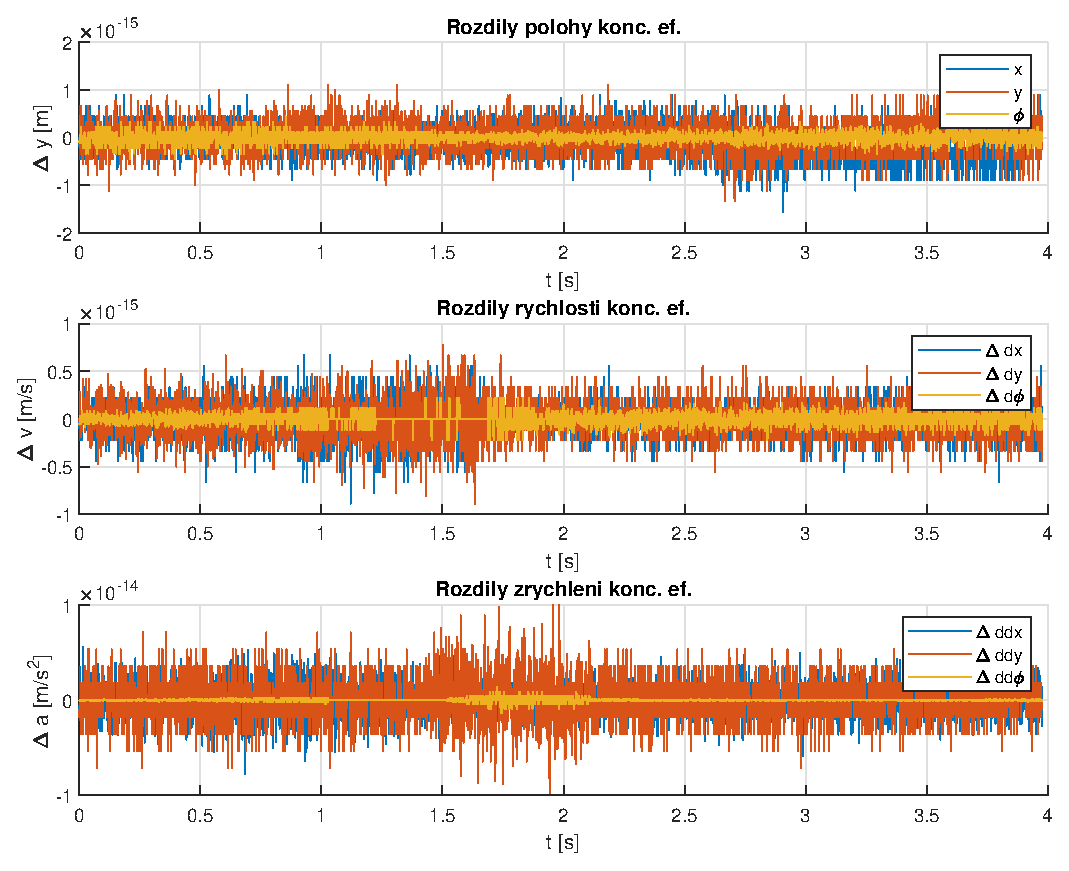
\includegraphics[width=\textwidth]{./Graphics/4_Graphics/Srovnani_POKU_model.eps}
					\caption{Ověření správnosti funkce POKU, IOKU vůči modelu vytvořenému v Simscape.}
					\label{graph:4_Srovnani_POKU_model}
				\end{figure}
			Z průběhu generátoru trajektorie koncového efektoru \textbf{MCS*} lze vypozorovat plánovaný pohyb daný body \textbf{A}, \textbf{B}, \textbf{C} a poloměrem \(r\). Na obrázku \ref{graph:4_Gen_vystup} je zřetelně vidět změna průběhu souřadnice x, jejíž vrchol je přibližně středem kruhové části trajektorie. Při pohledu na rychlosti a zrychlení v témže obrázku je zřejmé z výkyvů grafů, kde konkrétně se efektor pohybuje po kružnici, protože pro lineární pohyb po přímkách zůstávají derivace konstantní. Vykreslená data tedy odpovídají našemu předpokladu.\\
				\begin{figure}[H]
					\centering
					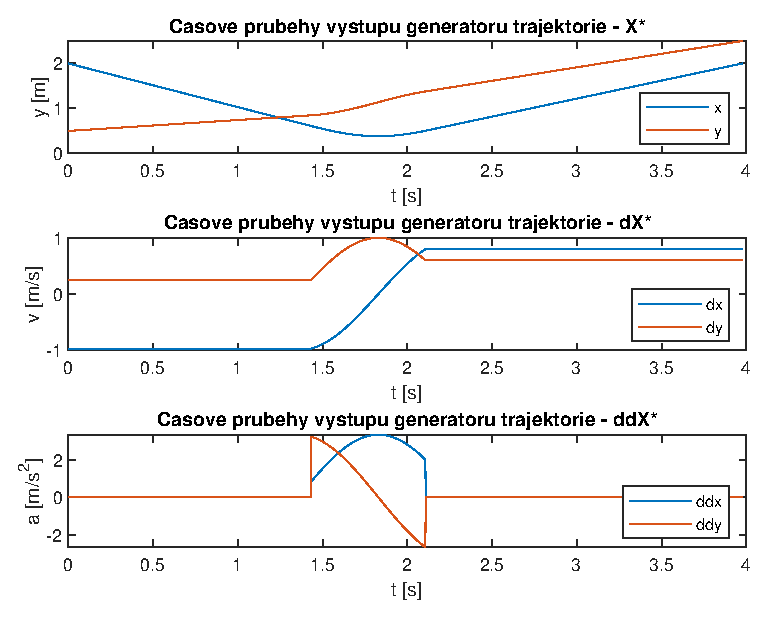
\includegraphics[width=\textwidth]{./Graphics/4_Graphics/GEN_vystup.eps}
					\caption{Časové průběhy zobecněných souřadnic generované generátorem trajektorie s jejich derivacemi.}
					\label{graph:4_Gen_vystup}
				\end{figure}
			
			Manipulátor však pro uskutečnění požadované trajektorie potřebuje kloubové souřadnice a jejich derivace, které nám poskytne na základě \textbf{MCS*} funkce \textbf{IOKÚ} v podobě matice \textbf{ACS}. Její průběh je v obrázku \ref{graph:4_Kloub_souradnice} a jako u výstupu generátoru lze pozorovat podobné chování ve stejných fázích simulace. Můžeme tedy tvrdit, že průběh kloubových souřadnic je geometricky správný s odvoláním i na graf výstupu modelu (viz obrázek \ref{graph:4_Srovnani_POKU_model}).\\
				\begin{figure}[H]
					\centering
					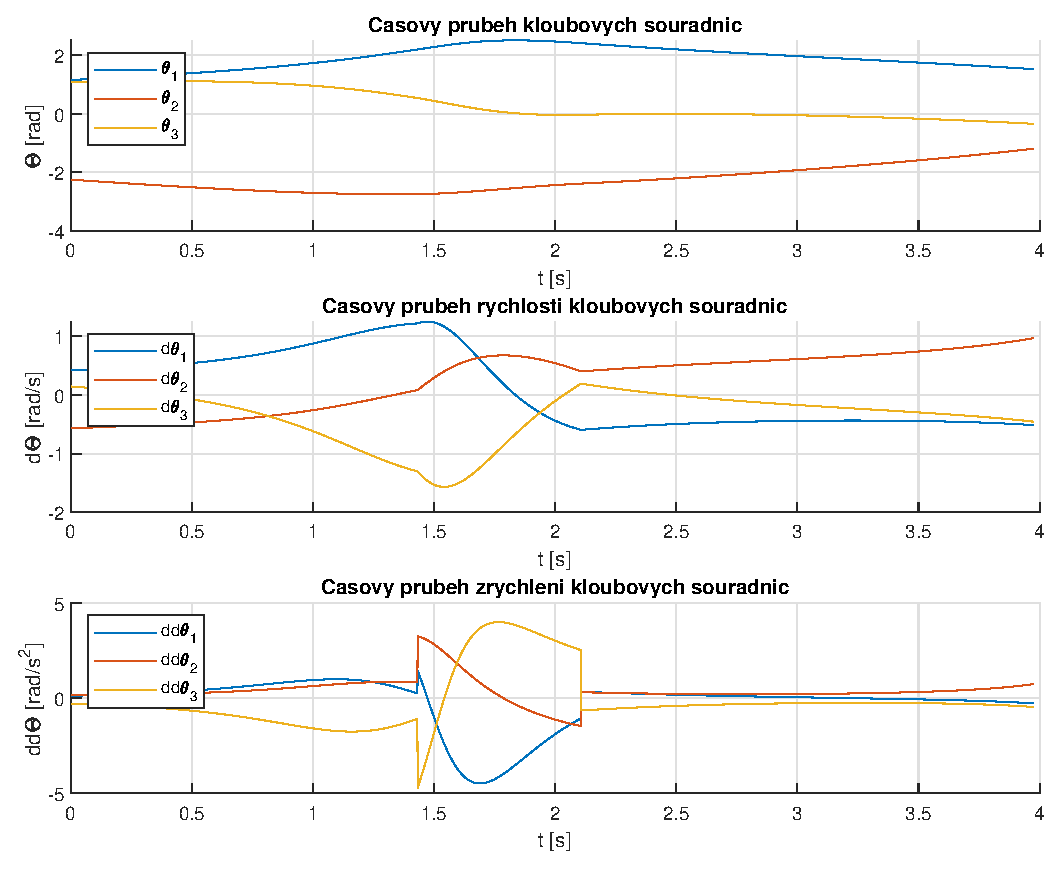
\includegraphics[width=\textwidth]{./Graphics/4_Graphics/Kloub_souradnice.eps}
					\caption{Průběh kloubových souřadnic při volbě konstantního \(\varphi = 0\).}
					\label{graph:4_Kloub_souradnice}
				\end{figure}
			Za použití vzorečku \[v = \sqrt{\dot{x}^2+\dot{y}^2}\] získáme rychlost pohybu koncového efektoru po požadované dráze, která je vykreslena v obrázku \ref{graph:4_vmax_overeni} jako rozdíl \(v-v_{max}\), kde \(v_{max}=1\). Jak lze vidět, odchylky jsou velmi malé a podmínku dodržení konstantní maximální rychlosti jsme zde splnili.\\
				\begin{figure}[H]
					\centering
					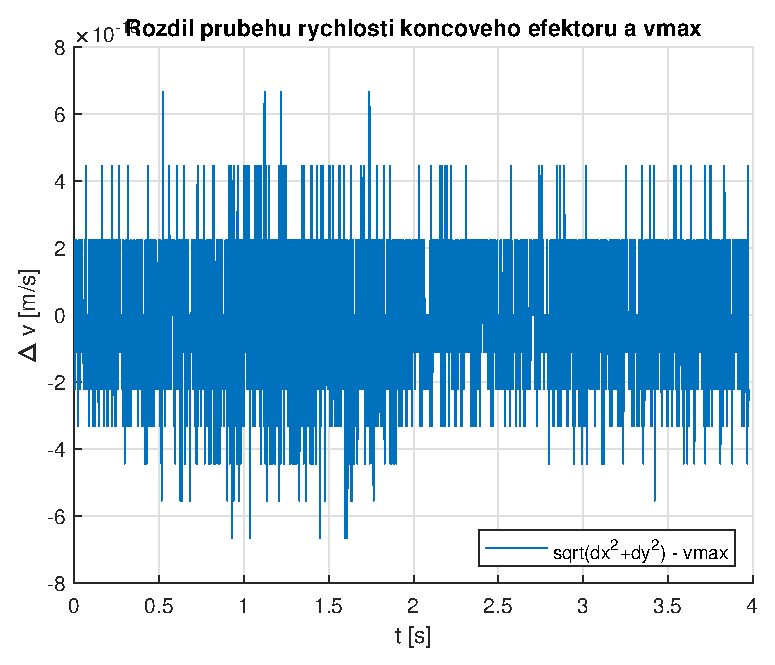
\includegraphics[width=\textwidth]{./Graphics/4_Graphics/vmax_overeni.eps}
					\caption{Ověření rychlosti koncového efektoru vůči požadovanému \(v_{max}\).}
					\label{graph:4_vmax_overeni}
				\end{figure}
		\subsection{Závěr}
			Na základě poskytnutého odvození parametrizace trajektorie se nám podařilo úspěšně sestavit generátor trajektorie, který poskytuje geometricky správné hodnoty. Použitím funkcí \textbf{IOKÚ} a \textbf{POKÚ} z předchozího zadání v sekci \ref{section:3} se nám povedlo rozhýbat manipulátor, který se pohyboval správně podle vygenerované trajektorie s minimálními odchylkami viz. \nameref{section:4_vysledky}.
	\newpage	
	\section{Singulární polohy manipulátoru}
		\subsection{Zadání}
			Následující úkoly řešte pro manipulátor zadaný v úloze \ref{section:2}
				\begin{enumerate}
					\item Vypočtěte podmínku pro kloubové souřadnice manipulátoru pro robot nacházející se v singulární poloze a diskutujte geometrické uspořádání robotu v této poloze.
					\item Znázorněte singulární polohu manipulátoru v prac. prostoru - rovině \(xy\) parametrizované zobecněnou souřadnicí \(\Phi\).
				\end{enumerate}
		\subsection{Postup řešení}
			Ze znalosti podmínky singulární polohy 
				\begin{align}
					det(J)=0,
				\end{align}
			kde \(J\) je analytický (kinematický) jakobián. Získáme ho parciální derivací jako 
				\begin{align}
					J(Q) =\frac{\delta F(Q)}{\delta Q}
				\end{align}
			kde 
				\begin{align}
					F(Q)=X=\begin{bmatrix}x\\ y\\ \varphi\end{bmatrix}
				\end{align}
			a 
				\begin{align}
					Q=\begin{bmatrix}\Theta_{1}\\ \Theta_{2}\\ \Theta_{3}\end{bmatrix}.
				\end{align}
			Jinými slovy lze mluvit o vektoru zobecněných souřadnic koncového efektoru \(X\) a kloubovými souřadnicemi \(Q\). Vektor \(X\) lze získat snadno pomocí metody \textbf{DGM} a skládání homogenních transformačních matic podle D-H úmluvy. Po dosazení nulových hodnot namísto posunu v ose \(z\), natočení kolem osy \(x\) a vyjádření zobecněných souřadnic získáme obecně vyjádřený vektor 
				\begin{align}
					X=\begin{bmatrix}x\\ y\\ \varphi\end{bmatrix}=\begin{bmatrix}
					a_2 \,\cos \left(\Theta_1 +\Theta_2 \right)+a_1 \,\cos \left(\Theta_1 \right)+a_3\,\cos\left(\Theta_1 +\Theta_2 +\Theta_3 \right)\\
					a_2 \,\sin \left(\Theta_1 +\Theta_2 \right)+a_1 \,\sin \left(\Theta_1 \right)+a_3\,\sin\left(\Theta_1 +\Theta_2 +\Theta_3 \right)\\
					\textrm{atan2}\left(\sin \left(\Theta_1 +\Theta_2 +\Theta_3 \right),\cos \left(\Theta_1+\Theta_2+\Theta_3 \right)\right)
					\end{bmatrix},
				\end{align}
			kde vektor \(\begin{bmatrix}a_{1}\\ a_{2}\\ a_{3}\end{bmatrix} = \begin{bmatrix}2\\ 1.5\\ 0.5\end{bmatrix}\) obsahuje parametry manipulátoru, což jsou dle D-H úmluvy posuny v osách \(x\) neboli parametry \(a_{i}\).\\
			Nyní již pouze dle výše zmíněných parciálních derivací \(F(Q)\) podle vypočteme jakobián viz rovnice (\eqref{eq:jacobian}) 
				\begin{align}
					\begin{array}{c}J=
					\begin{bmatrix}
						-a_2 \,\sin \left(\Theta_1 +\Theta_2 \right)-a_1 \,\sin \left(\Theta_1 \right)-\sigma_1  &-a_2 \,\sin \left(\Theta_1 +\Theta_2 \right)-\sigma_1  & -\sigma_1 \\
						a_2 \,\cos \left(\Theta_1 +\Theta_2 \right)+a_1 \,\cos \left(\Theta_1 \right)+\sigma_2  & a_2\,\cos \left(\Theta_1 +\Theta_2 \right)+\sigma_2  & \sigma_2 \\
						1 & 1 & 1
					\end{bmatrix}\\
					\mathrm{}\\
					\mathrm{where}\\
					\mathrm{}\\
					\;\;\sigma_1 =a_3 \,\sin \left(\Theta_1 +\Theta_2 +\Theta_3 \right)\\
					\mathrm{}\\
					\;\;\sigma_2 =a_3 \,\cos \left(\Theta_1 +\Theta_2 +\Theta_3 \right)
					\end{array}.
				\end{align}
			Nyní vypočteme 
				\begin{align}
					det(J)=a_1 \,a_2 \,\sin \left(\Theta_1 +\Theta_2 \right)\,\cos \left(\Theta_1 \right)-a_1 \,a_2\,\cos \left(\Theta_1 +\Theta_2 \right)\,\sin \left(\Theta_1 \right)
				\end{align}
			a po zjednodušení goniometrických funkcí dostaneme výraz 
				\begin{align}
					det(J)=a_1 \,a_2 \,\sin \left(\Theta_2 \right)
				\end{align}
			a dále jen položíme roven nule, abychom zjistili, pro jaké hodnoty existují singulární polohy. Jelikož \(a_{1}\) a \(a_{2}\) jsou konstantní parametry manipulátoru, singulární polohy definuje kloubový úhel \(\Theta_{2}\). Ze znalosti funkce \(sin\) víme, že 
				\begin{align}
					sin(\Theta_{2})=0 \; \text{pro}\; \Theta_{2} = 0 + k\cdot \pi, \;\text{kde k}\; \in \mathbb{Z}.
				\end{align}
			Pokud \(\Theta_{2}\) manipulátoru fixujeme v singulární poloze a za předpokladu požadovaného \(\varphi = 0\) koncového efektoru, zbývá nám jediný volitelný úhel \(\Theta_{1}\). Při této znalosti dosadíme do předpisu polohy koncového efektoru a jelikož je \(\varphi = \left(\Theta_{1}+\Theta_{2}+\Theta_{3}\right)\) konstantní, nebude se měnit a výraz se zjednoduší na dvě rovnice.
				\begin{align}
					\begin{array}{c}
						x = a_2 \,\cos \left(\Theta_1 +\Theta_2 \right)+a_1 \,\cos \left(\Theta_1 \right)+a_3\,\cos\left(\Theta_1 +\Theta_2 +\Theta_3 \right)\\
						y = a_2 \,\sin \left(\Theta_1 +\Theta_2 \right)+a_1 \,\sin \left(\Theta_1 \right)+a_3\,\sin\left(\Theta_1 +\Theta_2 +\Theta_3 \right)
					\end{array}
				\end{align}
			Po úpravě rovnic a dosazení dostaneme
				\begin{align}
					\begin{array}{c}
						x = a_2 \,\cos \left(\Theta_1 +\Theta_2 \right)+a_1 \,\cos \left(\Theta_1 \right)+a_3\,\cos\left(\varphi \right)\\
						y = a_2 \,\sin \left(\Theta_1 +\Theta_2 \right)+a_1 \,\sin \left(\Theta_1 \right)+a_3\,\sin\left(\varphi \right).
					\end{array}
				\end{align}
			Protože \(\Theta_{2}\) nabývá hodnoty \(0 + k\cdot \pi, \;\text{kde k}\; \in \mathbb{Z}\), můžeme výraz dále zjednodušit dosazením. Pokud je \(\Theta_{2} = 0\) nebo jeho \(2\pi\) násobkům, hodnota funkcí \(sin\) a \(cos\) nebude záviset na daném úhlu \(\Theta_{2}\). Dostaneme tak soustavu
				\begin{align}
					\begin{array}{c}
						x = a_2 \,\cos \left(\Theta_1\right)+a_1 \,\cos \left(\Theta_1 \right)+a_3\,\cos\left(\varphi \right)\\
						y = a_2 \,\sin \left(\Theta_1\right)+a_1 \,\sin \left(\Theta_1 \right)+a_3\,\sin\left(\varphi \right).
					\end{array}
				\end{align}
			Při dosazení \(\Theta_{2} = \pi\) nebo jeho \(2\pi\) násobků již dochází k permanentnímu posunu na jednotkové kružnici o \(\pi\), kde po přičtení druhého úhlu \(\Theta_{1}\) získáme opačné hodnoty funkcí \(sin\) a \(cos\). Při této znalosti však můžeme výraz zjednodušit vypuštěním úhlu \(\Theta_{2}\) a přidáním znaménka \(-\) před související goniometrické funkce. Hodnoty rovnic se tak pro dané \(\Theta_{2}\) nezmění a budou mít tvar
				\begin{align}
					\begin{array}{c}
						x = -a_2 \,\cos \left(\Theta_1\right)+a_1 \,\cos \left(\Theta_1 \right)+a_3\,\cos\left(\varphi \right)\\
						y = -a_2 \,\sin \left(\Theta_1\right)+a_1 \,\sin \left(\Theta_1 \right)+a_3\,\sin\left(\varphi \right).
					\end{array}
				\end{align}
			Protože obě soustavy se liší pouze ve znaménkách, budeme je nadále upravovat společně. Vytkneme
				\begin{align}
					\begin{array}{c}
						x = (a_1 \pm a_2) \,\cos \left(\Theta_1\right)+a_3 \,\cos\left(\varphi \right)\\
						y = (a_1\pm a_2) \,\sin \left(\Theta_1\right)+a_3 \,\sin\left(\varphi \right),
					\end{array}
				\end{align}
			osamostatníme jednotlivé goniometrické funkce
				\begin{align}
					\begin{array}{c}
						x -a_3 \,\cos\left(\varphi \right) = (a_1 \pm a_2) \,\cos \left(\Theta_1\right)\\
						y -a_3 \,\sin\left(\varphi \right)= (a_1\pm a_2) \,\sin \left(\Theta_1\right)
					\end{array}
				\end{align}
			a nakonec umocníme na druhou jednotlivé rovnice, sečteme a upravíme do výsledného tvaru
				\begin{align}
					\begin{array}{c}
						\left(x -a_3 \,\cos\left(\varphi \right)\right)^2 +\left(y -a_3 \,\sin\left(\varphi\right)\right)^2 = (a_1 \pm a_2)^2.
						\label{eq:rce_kruznice}
					\end{array}
				\end{align}
			Získali jsme tak rovnici kružnice se středem v bodě \(\begin{bmatrix}x\\y\end{bmatrix} = \begin{bmatrix}a_3 \,\cos\left(\varphi \right)\\a_3 \,\sin\left(\varphi \right)\end{bmatrix} = \begin{bmatrix}a_3\\0\end{bmatrix} = \begin{bmatrix}0.5 m\\0\end{bmatrix}\) a poloměr, který závisí na zvoleném \(\Theta_{2}\).\\
			\noindent
			Pro \(\Theta_{2}=0+k\cdot\pi \; ;k\in \mathbb{Z}\) je poloměr \(r = a_1 + a_2 = 2m + 1.5m = 3.5m\).\\
			\noindent
			Pro \(\Theta_{2}=\pi+k\cdot\pi \; ;k\in \mathbb{Z}\) je poloměr \(r = a_1 - a_2 = 2m - 1.5m = 0.5m\).\\
			
			Vzniklé kružnice nám vyjadřují singulární polohy pro měnící se jediný volný parametr \(\Theta_{1}\) a konstantní \(\varphi = 0\).	Jelikož jsou výsledkem dvě kružnice, které mají stejný střed v bodě \(S\) a rozdílný poloměr, můžeme je vykreslit jako soustředné kružnice \(k1\) a \(k2\).\\
			
			Pokud by jsme hodnotu \(\varphi\) změnili na jiný úhel než \(0\) došlo by u rovnice \ref{eq:rce_kruznice} ke změně polohy středů soustředných kružnic, jejihž velikost by se však nezměnila, protože poloměry jsou dány fyzickými parametry manipulátoru (zde rameny \(a_{1}\) a \(a_{2}\)).
		\subsection{Výsledky}
			Když se podíváme na obrázek \ref{pic:singularni_poloha_nula}, kde je vykreslen manipulátor pro \(\Theta_{2}=0\), můžeme vidět, že jedna singularita nastává při úplném natažení prvních dvou ramen. Bude tak působit problémy zejména při pohybu koncového efektoru daleko báze manipulátoru.\\
			
			Druhá možnost uspořádání je pro \(\Theta_{2}=0\) vyobrazena jako složená první dvě ramena na obrázku \ref{pic:singularni_poloha_pi}. Z toho můžeme usoudit, že problematická bude manipulace velmi blízko bázi.
			Další možnosti úhlu \(\Theta_{2}\) dle výše popsané rovnice budou vést na tyto dvě pozice, kdy jsou první dvě ramena rovnoběžná buď ve složeném stavu a nebo plně nataženém.\\
			
			Díky nalezeným singularitám lze zpětně vidět na již vykreslených grafech z předešlých zadání, že při blízkosti \(\Theta_{2}\) jedné ze singulárních poloh mají rychlosti a zrychlení kloubových souřadnic větší výkyvy než kdyby tomu tak nebylo (viz následující zadání).\\
			
			Na následujících obrázcích \ref{pic:singularni_poloha_nula} a \ref{pic:singularni_poloha_pi} můžeme vidět uspořádání ramen manipulátoru v singulárních polohách a jejich odpovídající kružnice singularit \(k1\) a \(k2\) pro případ, kdy \(\varphi = 0\).
				\begin{figure}[H]
					\centering
					\includegraphics[width=\textwidth]{./Graphics/5_Graphics/singularni_poloha_nula.eps}
					\caption{Manipulátor v singulární poloze pro \(\Theta_2 = 0 +k\cdot2\pi \; ;k\in \mathbb{Z}\).}
					\label{pic:singularni_poloha_nula}
				\end{figure}
				\begin{figure}[H]
					\centering
					\includegraphics[width=\textwidth]{./Graphics/5_Graphics/singularni_poloha_pi.eps}
					\caption{Manipulátor v singulární poloze pro \(\Theta_2 = \pi +k\cdot2\pi \; ;k\in \mathbb{Z}\).}
					\label{pic:singularni_poloha_pi}
				\end{figure}
		\subsection{Závěr}
			Pro zadaný manipulátor jsme byli schopni díky podmínce singularity určit, že nastává pro \(\Theta_2 = 0 +k\cdot\pi \; ;k\in \mathbb{Z}\) a identifikovat tak problém předchozí úlohy, kdy docházelo k velkým výkyvům v rychlostech a zrychlení kloubových souřadnic. Po zafixování jsme získali rovnice pro dvě soustředné kružnice popisující polohu singulárních poloh v prostoru manipulátoru.
	\section{Orientace koncového efektoru}
		\subsection{Zadání}
			\begin{figure}[H]
				\centering
				\includegraphics[width=\textwidth]{./Graphics/6_Graphics/6_zadani}
			\end{figure}
		\subsection{Postup řešení}
			Vzorec pro normu vektoru rychlostí je ${\mathbb{\dot{Q}}} = \sqrt{\dot{\theta_1}+\dot{\theta_2}+\dot{\theta_3}}$ V následujícím grafu na obrázku \ref{pic:Norma_vekt_dQ} můžeme vidět 3D graf generovaný pro jednotlivé konstantní úhly \(\varphi\) koncového efektoru po celé dráze pohybu efektoru \(s\). Vzniká zde viditelná nerovnost v podobě vysokých rychlostí kloubových souřadnic signalizující blízkost singulární polohy.
				\begin{figure}[H]
					\centering
					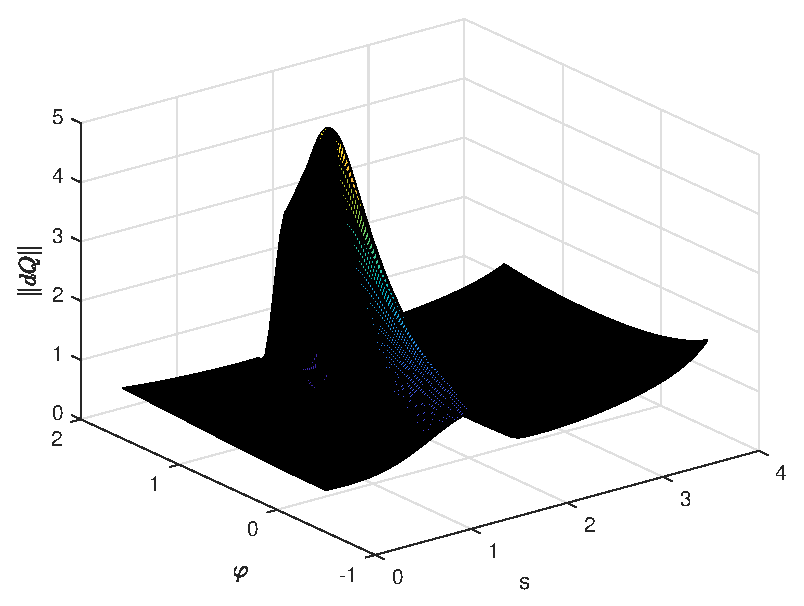
\includegraphics[width=\textwidth]{./Graphics/6_Graphics/Norma_vekt_dQ_konst.eps}
					\caption{Norma vektoru ${\mathbb{\dot{Q}}}$ pro konstantní úhly \(\varphi \in \langle -0.5, \frac{\pi}{2} \rangle\) pro dráhu pohybu \(s \in \langle 0, s_{max}\rangle\).}
					\label{pic:Norma_vekt_dQ}
				\end{figure}
			\subsubsection{Lineární interpolace}
				Požadavek na orientaci efektoru byl doposud konstantní úhel. V tomto bodu máme za úkol tento úhel lineárně měnit mezi dvěma předem zadanými úhly. Pro výpočet jsme použili následující rovnice 
					\begin{align}
						\varphi(t) = \varphi_s+\frac{s(t)}{s_{max}}\cdot(\varphi_e-\varphi_s)
					\end{align}
				dále platí
					\begin{align}
						\dot{\varphi}(t) = \varphi_s+\frac{v(t)}{s_{max}}\cdot(\varphi_e-\varphi_s)\\
						\Ddot{\varphi}(t) = \varphi_s+\frac{a(t)}{s_{max}}\cdot(\varphi_e-\varphi_s)
					\end{align}
				Na následujícím obrázku \ref{pic:Norma_vekt_dQ_lin} lze vidět, jak vypadá průběh normy rychlostí kloubových souřadnic pro lineární změnu \(\varphi\) od úhlu \(\frac{\pi}{2}\) až do \(0\). Při průběhu z počátečního úhlu do koncového je však manipulátor vystaven vysokým rychlostem kloubových souřadnic díky pohybu blízko singulární poloze. Pokud by se celý průběh v prostoru posunul do místa s nižšími hodnotami norem rychlostí, omezili bychom tak namáhání manipulátoru a výkonnostní požadavky na motory. Naštěstí lze změnit průběh úhlu \(\varphi\) tak aby se vyhnulo právě oblastem s vyššími hodnotami norem viz níže.
					\begin{figure}[H]
						\centering
						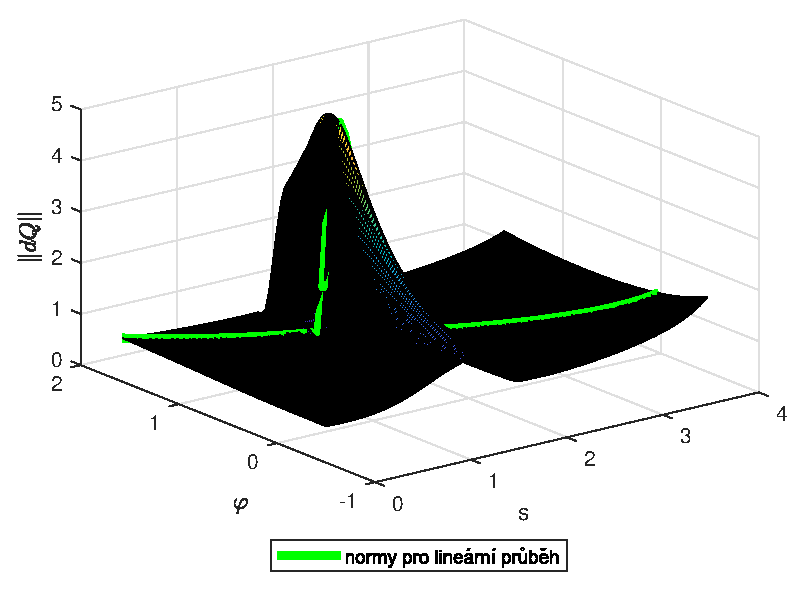
\includegraphics[width=\textwidth]{./Graphics/6_Graphics/Norma_vekt_dQ_lin3D.eps}
							\caption{Norma vektoru $\mathbb{Q}$ pro lineárně definované $\varphi$.}
						\label{pic:Norma_vekt_dQ_lin}
					\end{figure}
					\begin{figure}[H]
						\centering
						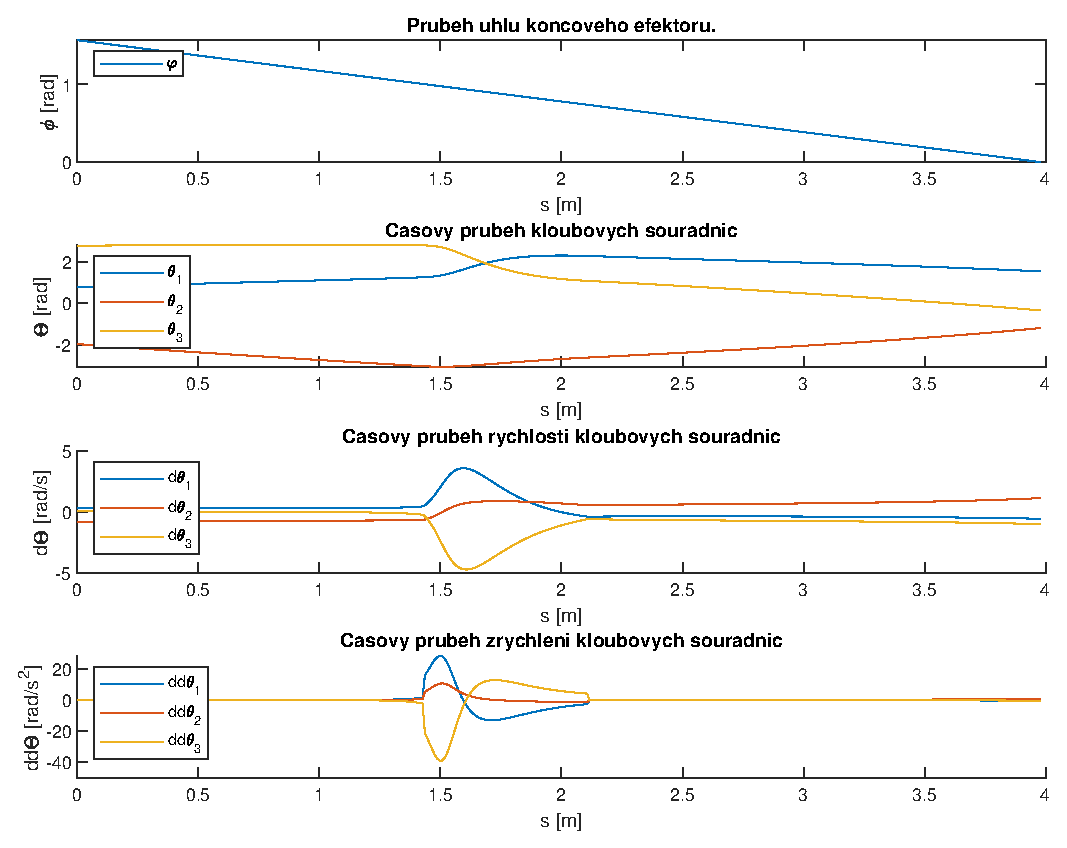
\includegraphics[width=\textwidth]{./Graphics/6_Graphics/Kloub_souradnice_lin.eps}
						\caption{Matice ACS pro lineárně definovaný úhel \(\varphi\).} 
					\end{figure}
					\newpage
			\subsubsection{Kvadratická interpolace}	
					Abychom zabránili neplynulému pohybu, který je způsobený singulárními polohami a vyhnuli se tak oblastem s vysokými hodnotami norem rychlostí, navrhli jsme kvadratickou interpolaci. Při tomto postupu se nám podaří zachovat startovní a koncový úhel beze změny, pouze pohyb mezi nimi nebude probíhat po lineární, ale kvadratické křivce, která je popsána následujícími rovnicemi
						\begin{align}
						\varphi = a_1s^2+a_2s+a_3\\
						\dot{\varphi} = 2a_1s+a_2\\
						\ddot{\varphi} = 2a_1
					\end{align}
				Koeficienty polynomu jsme matematicky vyjádřili, což nám umožňuje flexibilitu ve volbě středového průběžného bodu, kterým křivka bude procházet. Průběžný bod jsme zvolili v polovině délky celkové dráhy pohybu koncového efektoru a o velikosti úhlu rovný násobku \(-\frac{1}{3}\) startovního úhlu. Dosáhli jsme tak výrazného snížení požadavků na rychlosti pohybu kloubových motorů, což je vidět z průběhu kloubových souřadnic na obrázku \ref{pic:6_kloubove souradnice_quad}. Zároveň jsme se tak vyhnuli vysokým normám rychlostí volbou vhodnějšího průběhu z počátečního do koncového úhlu než při lineární změně viz. obrázek \ref{pic:6_vsechny normy}.
			\begin{figure}[H]
				\centering
				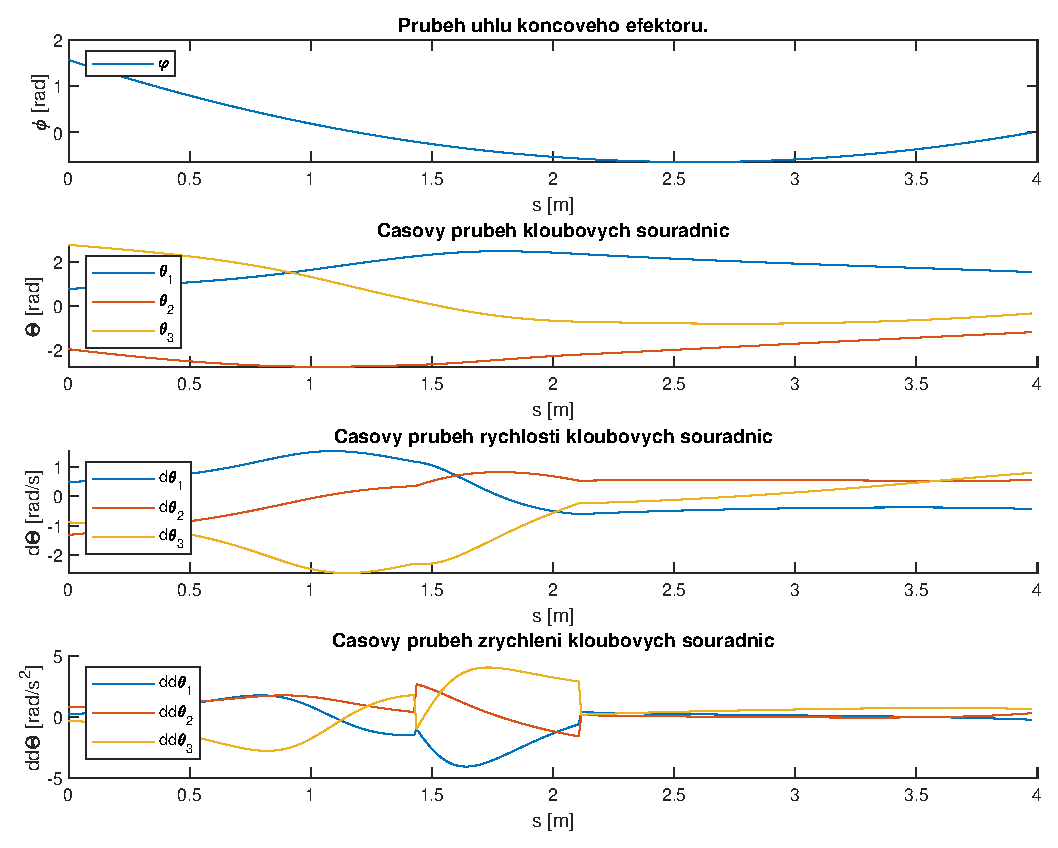
\includegraphics[width=\textwidth]{./Graphics/6_Graphics/Kloub_souradnice_quad.eps}
				\caption{Matice ACS pro kvadratický model}
				\label{pic:6_kloubove souradnice_quad}
			\end{figure}
			\begin{figure}[H]
				\centering
				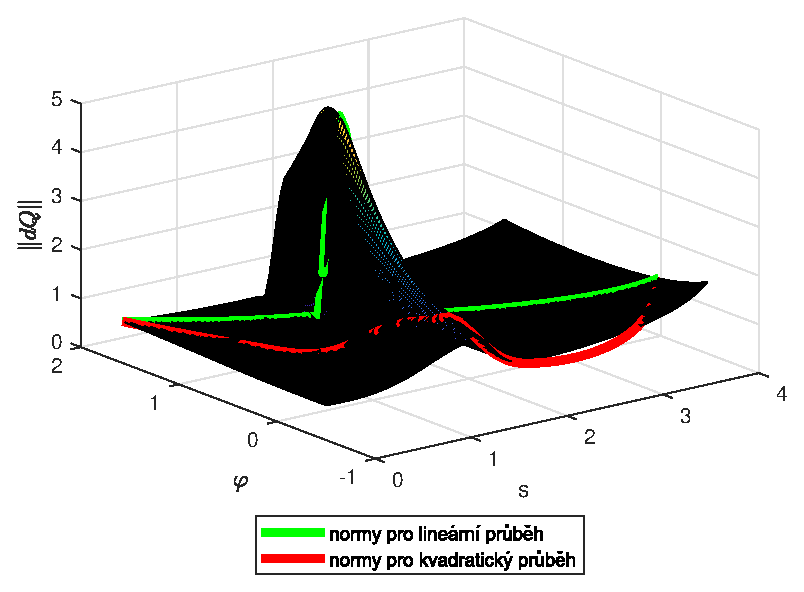
\includegraphics[width=\textwidth]{./Graphics/6_Graphics/Norma3d_vekt_dQ_vse.eps}
				\caption{Porovnání průběhu norem rychlostí v okolí singulárního bodu při lineárním a kvadratickém průběhu \(\varphi\)}
				\label{pic:6_vsechny normy}
			\end{figure}
		\subsection{Závěr}
		Hodnota normy nám ukázala že v rozsahu $<0,s_{max}>$ při úhlu otáčení $\varphi \in(-0.5,\frac{\pi}{2})$ dochází k největší změně úhlových rychlostí přibližně ve vteřině a půl. Tento bod je přibližně střed trajektorie ze zadání, kde jsme také zvolili průběžný bod pro kvadratickou interpolaci. 
		\par 
		Z grafů lze vidět že při přiblížení k singulární poloze dojde k prudkému nárůstu zrychlení v kloubech. Toto je pro reálný manipulátor nepřípustné, jelikož by mohlo dojít k jeho nadměrnému namáhání případně poškození.
		Tento jev jsme eliminovali pomocí kvadratické interpolace. Z grafů lze vidět zásadní zlepšení průběhů rychlostí i zrychlení při zachování stejných počátečních a koncových úhlů natočení konc. ef., což by v praxi mělo za následek lepší chování manipulátoru a jeho větší životnost.
		
		
\end{document}
